% IEEE Paper Template for US-LETTER Page Size (V1)
% Sample Conference Paper using IEEE LaTeX style file for US-LETTER pagesize.
% Copyright (C) 2006-2008 Causal Productions Pty Ltd.
% Permission is granted to distribute and revise this file provided that
% this header remains intact.
%
% REVISION HISTORY
% 20080211 changed some space characters in the title-author block
%
\documentclass[10pt,conference,letterpaper]{IEEEtran}
\usepackage{times,amsmath,epsfig}

\usepackage{graphicx}
\usepackage{algorithm} % for algorithms
\usepackage{algpseudocode}
\usepackage{booktabs} % For formal tables
%\usepackage{amsthm} % For claims  ???????

%
\title{An optimistic approach to handle out-of-order events within analytical stream processing}
%
\author{%
% author names are typeset in 11pt, which is the default size in the author block
{Igor E. Kuralenok{\small $~^{\#1}$}, 
    Nikita Marshalkin{\small $~^{\#2}$},
    Artem Trofimov{\small $~^{\#3}$}, 
        Boris Novikov{\small $~^{\#4}$} }%
% add some space between author names and affils
\vspace{1.6mm}\\
\fontsize{10}{10}\selectfont\itshape
% 20080211 CAUSAL PRODUCTIONS
% separate superscript on following line from affiliation using narrow space
$^{\#}$\,JetBrains Research\\
Saint Petersburg, Russia\\
\fontsize{9}{9}\selectfont\ttfamily\upshape
%
% 20080211 CAUSAL PRODUCTIONS
% in the following email addresses, separate the superscript from the email address 
% using a narrow space \,
% the reason is that Acrobat Reader has an option to auto-detect urls and email
% addresses, and make them 'hot'.  Without a narrow space, the superscript is included
% in the email address and corrupts it.
% Also, removed ~ from pre-superscript since it does not seem to serve any purpose
$^1$\,ikuralenok@gmail.com   %  \\
$^2$\,marnikitta@gmail.com    %  \\
$^3$\,trofimov9artem@gmail.com   % \\
$^4$\,borisnov@acm.org 
}
%
\newcommand{\PicScale}{0.5}
\newcommand {\FlameStream} {FlameStream}

\begin{document}
\maketitle
%
\begin{abstract} 
Abstract
\end{abstract}

% NOTE keywords are not used for conference papers so do not populate them
% \begin{keywords}
% keyword-1, keyword-2, keyword-3
% \end{keywords}
%
\section {Introduction}
%%% fs-seim-intro - Introduction

\label {fs-intro}

Nowadays, a lot of real-life applications use stream processing for network monitoring, financial analysis, training machine learning models, etc. State-of-the-art industrial stream processing systems, such as Flink \cite{carbone2015apache}, Samza \cite{Noghabi:2017:SSS:3137765.3137770}, Storm \cite{apache:storm}, Heron \cite{Kulkarni:2015:THS:2723372.2742788}, are able to provide low-latency and high-throughput in distributed environment for a wide range of analytical problems. However, issues related to the order-sensitive computations still remain. Most of these systems assume that events are fed to the system with monotonically increasing timestamps or with minor inversions. Often, such timestamps can be assigned at system's entry. Nevertheless, even if input items arrive at system's entry monotonically, they can be reordered because of parallel and asynchronous processing. In this case, order-sensitive operations located in data flow pipeline quite deeply can be broken. Figure ~\ref{break-order-dataflow} shows the example of common distributed stream processing pipeline that breaks the input order of operation, even if input events are monotonic and links between operations guarantee FIFO order. Basically, ordering constraints make sense only for stateful operations.

\begin{figure}[htbp]
  \centering
  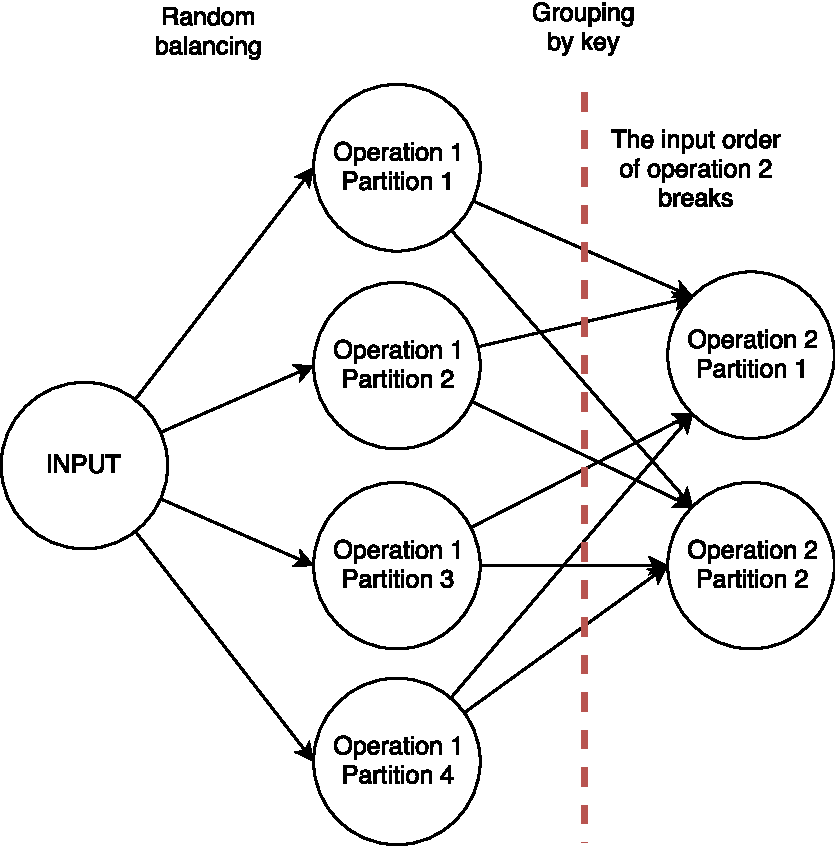
\includegraphics[width=0.38\textwidth]{pics/break_order_pipeline}
  \caption{An  example of common distributed stream processing pipeline that breaks the input order of operation}
  \label {break-order-dataflow}
\end{figure}

The typical way to achieve in-order processing is to buffer operation's input for some time to ensure that there are no out-of-order items. Most of the modern stream processing systems provide functionality to buffer all input items before specified operations until some user-provided conditions are satisfied. Conditions can be set on timing or the count of elements in the buffer. The main disadvantage of such techniques is that it can lead to significantly large latency, especially if the processing pipeline contains several operations that require ordered input. 

An alternative option is to handle out-of-order items as a special case in the business logic of operation. However, this way is suitable only for the limited number of tasks. Moreover, it may dramatically complicate the business-logic, which can lead to increasing the cost of its maintenance and is error-prone.
% sophisticated bugs.    

In this paper we propose an optimistic approach to handle out-of-order events in any stateful operation. In addition, we demonstrate its advantages compared to existing solutions. The contributions of this paper are the following: 

\begin {itemize}
\item Definition of new optimistic technique to handle out-of-order items in stateful operations
\item Demonstration of properties of this approach
\item Demonstration of working example that applies proposed method
\end {itemize}

The rest of the paper is structured as follows: in section~\ref{fs-stream} we formalize the preliminaries of stream processing, the examples of tasks that require ordered input are described in section~\ref{fs-tasks}, the typical approaches for handling out-of-order events are discussed in~\ref{fs-typical}, our optimistic technique is detailed in~\ref{fs-optimistic} and its performance is demonstrated in ~\ref{fs-experiments}, the main differences between proposed method and existing ones are shown in~\ref{fs-related}, finally we discuss the results and our plans in~\ref{fs-conclusion}.


\section{Stream processing dataflow}
%%% fs-seim-stream - Stream processing concepts

%%% TODO: replace event to item
%%% TODO: the/a figure 

\label {fs-stream}

In this section we define some preliminaries for distributed stream processing. It allows us to unify required terms and to introduce definitions, which are needed for the subsequent statements.

In this paper a stream processing system is considered as a shared-nothing distributed runtime. It handles input items and processes them one-by-one according to user-provided logic. It is able to handle a potentially unlimited number of items. The main requirement of this kind of data processing systems is to provide low latency between event occurrence and its processing under fixed load. The term {\em distributed} implies that user's procedures can be partitioned on distinct computational units or shards. The following subsections detail the properties of such systems more precisely.  

\subsection{Data flow}
The basic data flow abstraction is a {\it stream}. The stream is an infinite sequence of data items. Each data item contains a payload defined by a user. Besides, it can be accompanied by meta-information. Typically meta-information is used to define an order on data items. For instance, it can be represented as a UNIX timestamp in milliseconds.

%%% Trace?

\subsection{Computation flow}
Commonly, the computational pipeline is defined in the form of {\it logical graph}. The vertices of the logical graph are operations, and the edges are links between them. Logical graph defines only relations between operations, but it does not describe the physical deployment. The logical graph for the pipeline shown in figure~\ref{break-order-dataflow} is presented in the figure~\ref{break-order-dataflow-logical}

\begin{figure}[htbp]
  \centering
  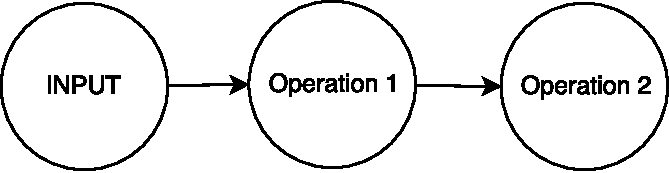
\includegraphics[width=0.38\textwidth]{pics/break_order_pipeline_logical}
  \caption{The logical graph for the physical graph shown above} 
  \label {break-order-dataflow-logical}
\end{figure}

\subsection{Operations}
There are two main types of streaming operations: {\it stateless} and {\it stateful}. Stateless operations do not need any knowledge about past inputs to correctly process current one. A simple illustration is a map operation that multiplies by 2 any numeric input item's payload. On the other hand, stateful operations are able to keep some aggregations or summaries of received events. In such case, the output of the operation depends not only on the input but also on its current state. As an example, one can define an operation that sums all previous items with numerical payloads.

\subsection{Physical deployment}
As mentioned above, each operation can be partitioned between multiple computational units. Data items can be balanced between partitions by key extracted from an item's payload for stateful operations. For stateless operations items can be balanced randomly. The schema of physical partitioning of operations is sometimes called {\it physical graph}. Regarding physical links between operations, in the most cases, it is assumed that they guarantee FIFO order.

\subsection{Guarantees}
Recognized important property of stream processing systems is the type of guarantees it provides in case of failures. There are three main types of such guarantees. {\it At most once} semantics states that each input event is processed once or not processed at all. {\it At least once} guarantees that each input item is processed, but possibly multiple times, that can lead to result duplication. {\it Exactly once} semantics guarantee that each input event is processed exactly one time.  


\section{Tasks that require in-order input}
%%% fs-seim-tasks - Tasks that require in-order input

\label {fs-tasks}

In this section we mention common problems that require the order of input items. Additionally, we note a couple of computation scenarios, which can be found in many real-life projects.

\subsection{Tasks requiring complete event retrieval}
Quite often we suppose that business-logic event is an atomic object, i.e. single data item. However, there are cases when single input event is split into multiple items within a stream. These input item derivatives can be processed independently, despite the fact that they all have the same meta-information. As it was shown in the figure ~\ref{break-order-dataflow}, independent processing can lead to reordering. Therefore, operations which require complete event data to process valid output cannot simply detect the completeness by the order of input items.

There are other solutions for this kind of problems rather than ordering of input items. They are shown in the section ~\ref{fs-typical}. 

\subsection{Tasks that depend on the order of input events}
This class includes all non-commutative operations. Such tasks strictly requires the order of input items, because there are no any other techniques to compute a valid result.

\subsection{Examples}

\subsubsection{???}

\subsubsection{Inverted index}
Pipeline shown in the figure ~\ref{break-order-dataflow} can be used for computing inverted index. In this case, operation 1 accepts documents from input and for each word produces corresponding positions. Operation 2 accepts pairs of word and positions and computes change log of inverted index for each word. Because of the fact that output change logs must be ordered in order to get valid index after applying them, operation 2 requires ordered input. 


\section{Typical solutions}
%%% fs-seim-typical - Typical solutions

\label {fs-typical}

There are two  most common methods that are used to implement order-sensitive operators: in-order processing (IOP) \cite{Arasu:2006:CCQ:1146461.1146463, Cranor:2003:GSD:872757.872838, hammad2004optimizing} and out-of-order processing (OOP) \cite{Li:2008:OPN:1453856.1453890}.

\subsection{IOP}

According to IOP approach, each operation must enforce the total order on elements. Simple operators, such as projection and selection, apply function and propagate output items down the stream without any additional buffering. However, even stateless operations may require buffering. Figure~\ref{iop} shows the union operation that combines multiple streams into the one. Both input streams are ordered, as predecessors must meet ordering constraint. Nevertheless, if there is arrival time skew between input streams, the union must buffer the earlier stream to produce ordered output. It is known that IOP is memory demanding and has unpredictable latencies and limited scalability \cite{Li:2008:OPN:1453856.1453890}.

\begin{figure}[htbp]
  \centering
  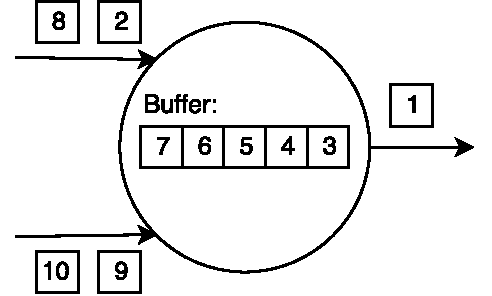
\includegraphics[width=0.30\textwidth]{pics/iop}
  \caption{IOP union operation. Due to delay of the upper stream operation must buffer elements}
  \label {iop}
\end{figure}

\subsection{OOP}

OOP is an architecture of streaming systems that does not require order maintenance if it is not needed. In the case of ordering requirements, OOP buffers input items similar to the IOP approach. To flush buffers, OOP systems use progress indicators such as punctuations \cite{Tucker:2003:EPS:776752.776780}, low watermarks \cite{Akidau:2013:MFS:2536222.2536229}, or heartbeats \cite{Srivastava:2004:FTM:1055558.1055596}. They go through the stream as ordinal items, but do not trigger business-logic of operations. Each punctuation carries meta-information and promises that there are no any elements with lesser meta-information. Therefore, punctuations must be monotonic, but data items between two consecutive punctuations can be arbitrarily reordered. Punctuations are periodically yielded by data sources.

A timed window operation can be mentioned   aas an example of OOP approach.  A window operation buffers partial aggregates until a punctuation for specific time arrives. After that,the  window flushes corresponding buffers and propagates the punctuation to the next operation down the stream.

OOP resolves some of the downsides of the IOP but it has several flaws too. Even if the input stream is totally ordered, the operation must wait for the punctuation. Figure~\ref{oop} illustrates such case. Bottom window is complete but must be blocked until the punctuation for item 11 arrives. Another issue of OOP is that periodical flushes can result in load bursts and increase of latency. 

\begin{figure}[htbp]
  \centering
  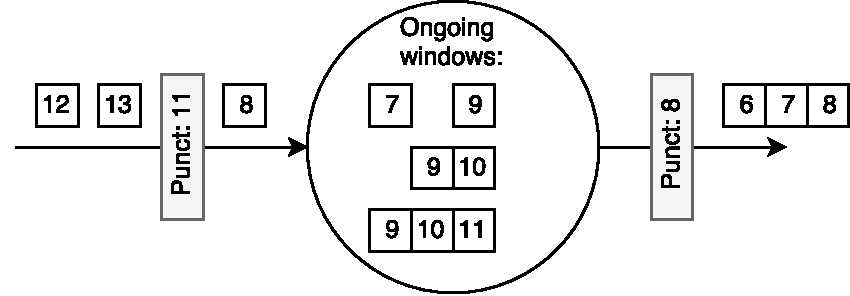
\includegraphics[width=0.48\textwidth]{pics/oop}
  \caption{OOP sliding window, range=3, slide=1. Operation must block lower window until next punctuation arrival }
  \label {oop}
\end{figure}


\section{Optimistic approach}
%%% fs-seim-optimistic - Optimistic approach

\label {fs-optimistic}

The main idea of our method is to represent stateful transformations as a sequence of a map and windowed grouping operations and handle out-of-order items within them. 

Following our approach, we make some assumptions about stream processing system, that is suitable for applying it. Such system must support meta-information on data items, allow cycles in the logical graph, and its set of predefined operations must be sufficient to express map and windowed grouping operations. Additionally, it should provide functionality to periodically promise that there are no any data items with meta-information less than specified.

In this section, firstly, we define the ordering model of data items. Then, we show that any stateful transformation can be implemented using the combination of windowed grouping and map operations. After that, we demonstrate an optimistic approach to handle out-of-order items within these operations. In the end of the section, the limitations of such technique are discussed.

\subsection{Ordering model}
We assume that there is a total order on meta-information of data items. Besides, ordering is preserved, when an item is going through the operations. More precisely, the order of output items is the same as the order of corresponding input items. Moreover, the output follows corresponding input but precedes the next item. The ordering model is shown in the figure ~\ref{ordering}.

\begin{figure}[htbp]
  \centering
  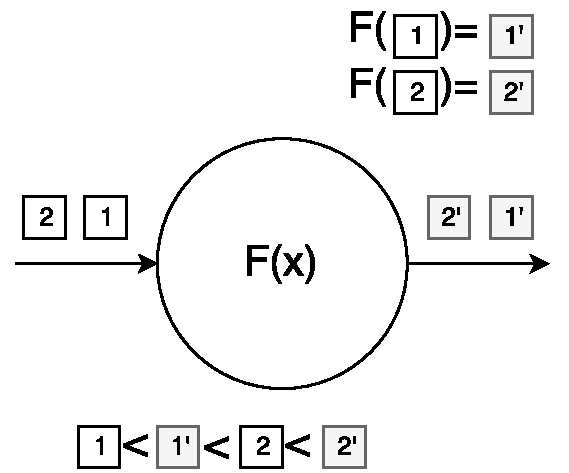
\includegraphics[width=0.48\textwidth]{pics/ordering}
  \caption{Ordering}
  \label {ordering}
\end{figure}

\subsection{Semantics of map and windowed grouping operations}

\subsubsection{Map}
Map transforms input item into a sequence of its derivatives, according to a function on item's payload provided by a user. This sequence can consist of any number of items or even be empty.

\subsubsection{Windowed grouping}
Windowed grouping is a stateful operation with a numeric parameter {\it window}. It is supposed that payloads of input items of grouping operation have key-value form. The state of this operation is represented by a set of buckets, one for each key. Windowed grouping has the following semantics:

\begin{itemize}
    \item Each input item is put into the corresponding bucket at position defined by its meta-information
    \item The output of grouping operation is a window-sized tuple of the last items in the corresponding bucket. If bucket size is less than window, the output contains full bucket
\end{itemize}

The following example illustrates the semantics of the windowed grouping operation. In this example, payloads of input items are represented as natural numbers: 1, 2, 3, etc. The hash function returns 1 if the number is even and 0 otherwise. If the window is set to 3, the output is:

\[(1), (2), (1|3), (2|4), (1|3|5), (2|4|6), (3|5|7), (4|6|8)...\]

\subsection{Stateful transformations using defined operations}
Figure ~\ref{stateful-schema} shows the part of the logical pipeline, that can be used for stateful transformation. The input of windowed grouping operation is supposed to be ordered. There are several functional steps to produce output and update state. These steps can be detailed by considering two cases:

\begin{itemize}
    \item When the first item arrives at grouping, it is inserted into the empty bucket. Grouping outputs single-element tuple, and then it is sent to the combined map. Combined map generates state object and sends it back to the grouping in the form of an ordinal key-value data item. The key of the state item is the same as in the item in tuple and value is the state. Combined map can generate some additional output and send it further down the stream
    \item When new regular input item arrives at windowed grouping, it is inserted into the corresponding bucket's tail, because of the order assumptions. Additionally, the right ordering guarantees that input item is grouped into the tuple with previously generated state item. The next map operation combines new item and previous state into the new state item. After that, the new state item is returned to the grouping through the cycle. As in the preceding case, combined map can generate some additional output
\end{itemize}

\begin{figure}[htbp]
  \centering
  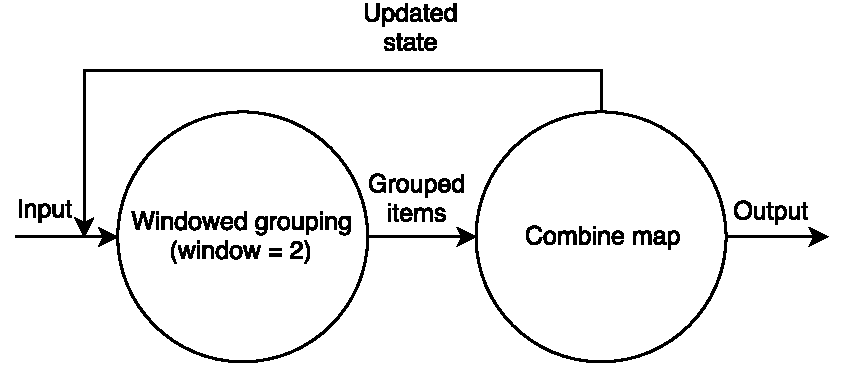
\includegraphics[width=0.48\textwidth]{pics/stateful-schema}
  \caption{The part of the logical pipeline for stateful transformation}
  \label {stateful-schema}
\end{figure}

The example of square matrix multiplication within proposed approach is shown in the figure ~\ref{matrix-example}. In this example, input items are represented as key-value pairs, where the key is the dimension of a matrix and the value is the matrix itself. The reaction on three input matrices are the following:

\begin{itemize}
    \item When the first matrix {\it A} arrives at grouping, it is put into the empty bucket for 3x3 matrices. After that, the single-element tuple with matrix {\it A} is sent to combine map operation. Combine map creates state object for matrix {\it A}, which is actually just {\it A} itself. In the last step, state item is sent back to grouping, and it is inserted right after item for matrix {\it A}
    \item Matrix {\it B} is arrived and inserted into the bucket right after state item. The tuple containing state item and item for matrix {\it B} is sent to combine map. Combine map multiplies matrix in the state by matrix {\it B}. The result of this operation is matrix {\it AB}. New state item for matrix {\it AB} is created and sent back to the grouping. It is inserted in bucket right after item with matrix {\it B}
    \item Matrix {\it C} is arrived and went through the pipeline in a similar way as matrix {\it B}
\end{itemize}

\begin{figure}[htbp]
  \centering
  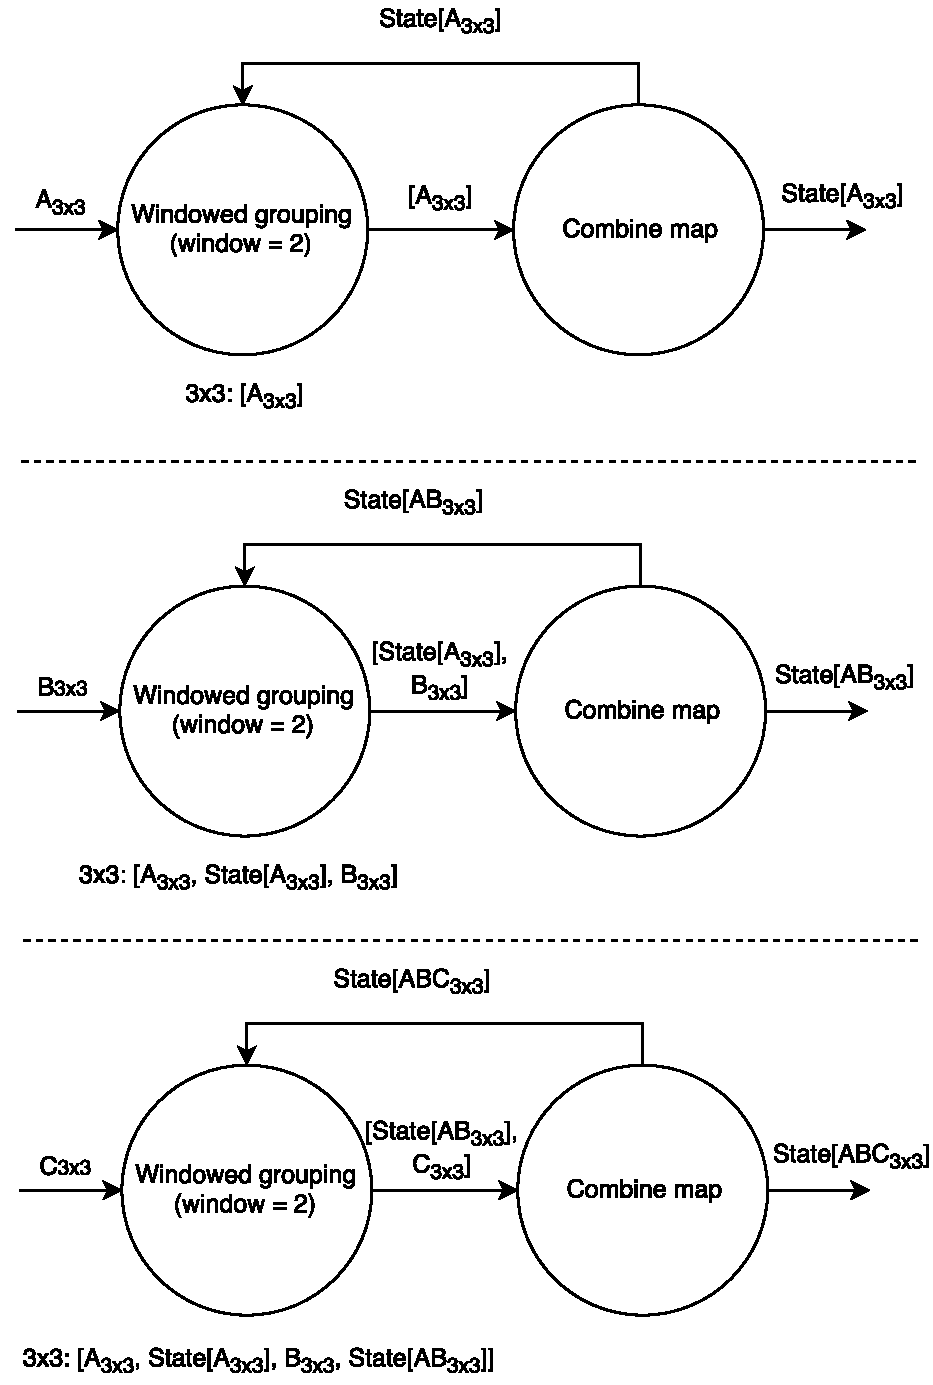
\includegraphics[width=0.48\textwidth]{pics/matrix-example}
  \caption{Matrix multiplication example}
  \label {matrix-example}
\end{figure}

\subsection{Handling out-of-order events}
When we introduce the model for stateful operations, we suppose that all items arrive at grouping in the right order. However, as it was shown above, it is not possible in practice without additional buffering due to the parallel and asynchronous processing. We propose the following approach to handle events in grouping:

\begin{itemize}
    \item If item arrives in order, it is processed as usual
    \item If item is out-of-order, then it is inserted into the corresponding position within the specified bucket. After that, tuples, which contain new item are generated and sent further down the stream. At the same time, tuples, that already has been generated, but became invalid, are generated again, but with a special flag in meta-information. This flag means that tuples with such meta-information are invalid, and they and their derivatives should not be sent to the user. Such elements are called {\it tombstones}. Tombstones have the same payloads as invalid items in order to go through the same path in the computational pipeline
\end{itemize}

The pseudocode of the grouping insertion is shown in algorithm \ref{group-insert}. The functions accept new element whether it ordinal item or tombstone and a bucket for element's hash. They call {\it Emit} function to send new items downstream.

\begin{algorithm*}
\caption{Grouping insertion}
\label{group-insert}
  \begin{algorithmic}[1]
    \Function{InsertTombstone}{$item$, $bucket$}
      
      \State $cleanPosition \gets lowerBound(item, bucket)$
      \ForAll{$group: group \cap cleanPosition \neq \emptyset$} 
        \State \Call{Emit}{$DataItem_{tomb}(group)$} \Comment{Send tombstones for invalid groups}
      \EndFor

      \State \Call{Remove}{$bucket, cleanPosition$}

      \ForAll{$group: group \cap cleanPosition \neq \emptyset$} 
        \State \Call{Emit}{$DataItem(group)$} \Comment{Emit new groups that appeared after collapse}
      \EndFor
    \EndFunction

    \item[]

    \Function{InsertRegular}{$item$, $bucket$}
      \State $insertPosition \gets lowerBound(item, bucket)$
      \ForAll{$group: group \cap insertPosition \neq \emptyset$} 
        \State \Call{Emit}{$DataItem_{tomb}(group)$} \Comment{Send tombstones for groups that would dissapear after insert}
      \EndFor
      
      \State \Call{Insert}{$bucket, insertPosition$}

      \ForAll{$group: group \cap insertPosition \neq \emptyset$} 
        \State \Call{Emit}{$DataItem(group)$} \Comment{Emit new groups}
      \EndFor
    \EndFunction
  \end{algorithmic}
\end{algorithm*}

This technique guarantees that all correct tuples are eventually produced. However, invalid items are also generated. Therefore, there is a need for {\it barrier} at the pipeline's sink ~\ref{graph-with-barrier}, that removes invalid output items, when corresponding tombstones arrive. The Barrier is partially flushed for some meta-information interval when there is a guarantee that there are no any out-of-order items and tombstones further up the stream for this interval. This guarantee can be provided by punctuations or low watermarks, as it is implemented in the most stream processing systems. 

The pseudocode for the barrier is shown in the algorithm  ~\ref{barrier-insert}. The function {\it Insert} is called upon new item's arrival, {\it Punctuation} - on punctuation's.

\begin{algorithm}
\caption{Barrier insertion}
\label{barrier-insert}
  \begin{algorithmic}[1]
    \State $buffer \gets \emptyset$

    \Function{Insert}{$item$}
      \State $position \gets lowerBound(item, buffer)$
      \If {$isTombstone(item)$}
        \State \Call{Remove}{$buffer, position$}
      \Else
        \State \Call{Insert}{$buffer, position$}
      \EndIf
    \EndFunction

    \item[]

    \Function{Punctuation}{$timestamp$}
      \ForAll{$item \in buffer : item_{timestamp} < timestamp$}
        \State \Call{Emit}{$item$}
        \State \Call{Remove}{$item$, $buffer$}
      \EndFor
    \EndFunction
  \end{algorithmic}
\end{algorithm}

The key idea behind this approach is to shift blocking as far as possible down the stream.

\subsection{Advantages and limitations}
The main advantage of the proposed technique is that items are processed optimistically, without waiting for the punctuation or low watermark. Therefore, when the watermark arrives, all computations can be already done, and there is only a need to flush barrier. Such approach can be especially efficient when stream computations are heavy and there are large time intervals between watermarks.

Regarding the weaknesses, this method can generate additional items, which can lead to extra network traffic. Experiments, that is shown in the section ~\ref{fs-experiments} demonstrates that in some cases the number of extra items is extremely low. However, if the task requires a very large number of out-of-order items, there is a need to analyze the applicability of proposed solution.




\section{Experiments}
%%% fs-seim-experiments - Experiments

\label {fs-experiments}

In order to estimate the performance, we implemented a prototype based on the proposed approach. As a stream processing task, we apply the computation of inverted index for 1000 Wikipedia documents. The logical pipeline of this computation is shown in Figure ~\ref{inverted-index}. First map operation accepts Wikipedia documents and outputs pairs of words and corresponding positions. The next part of the pipeline accepts pairs of word and positions and computes updated posting list and the actual changelog. 

This stateful transformation is implemented in the form of groping and map operation with a cycle, as it was shown in the previous section. Regarding the physical deployment, the full logical graph is deployed on each computational unit or worker. Documents are randomly shuffled before the first map operation. Word positions are partitioned by word before grouping. The other links are implemented as simple chain calls.

\begin{figure}[htbp]
  \centering
  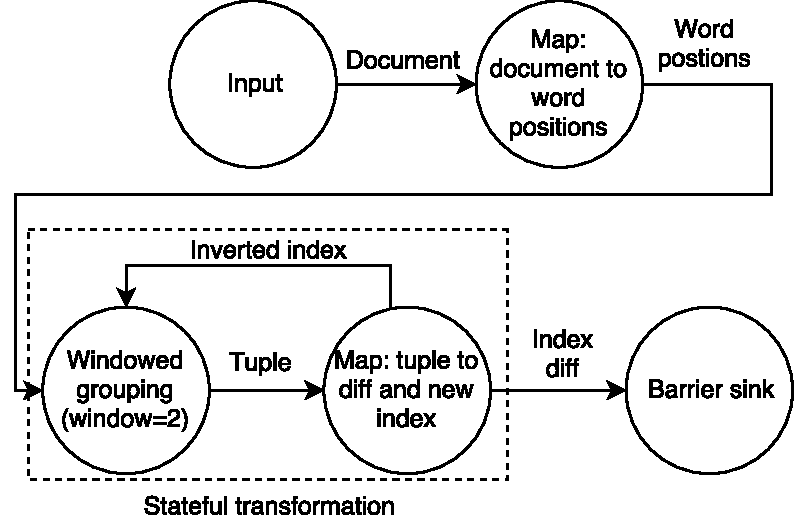
\includegraphics[width=0.48\textwidth]{pics/inverted-index}
  \caption{Logical pipeline for inverted index}
  \label {inverted-index}
\end{figure}

Our experiments were performed on clusters of 2, 4, 6, 8, and 10 nodes. Each node is an AWS EC2 micro instance with 1GB RAM and 1 core CPU.

As a key metric in our experiment, we take the ratio of arrived at the barrier items count to the number of the valid items among them. This value clearly represents the overhead of our approach, as it was mentioned at the end of the previous section. 

The relation between the number of workers, the delay between input documents and the proposed ratio is shown in Figure ~\ref{experiment}. As expected, the peak of the ratio is achieved when the document per second rate is high and the number of the nodes is low. This behaviour can be explained by the fact that a few workers cannot effectively deal with such intensive load. Nevertheless, the proportion of invalid items reduces with the increase of workers number. Under non-extreme load, the total overhead of the optimistic approach is under 10\% for all considered number of workers. These results confirm that the ratio does not increase with the growth of the number of nodes.

Therefore, the most important conclusions of the experiments are: the proposed method is scalable, the overhead could be optimized by system setup.

%% TODO: 
\begin{figure}[htbp]
  \centering
  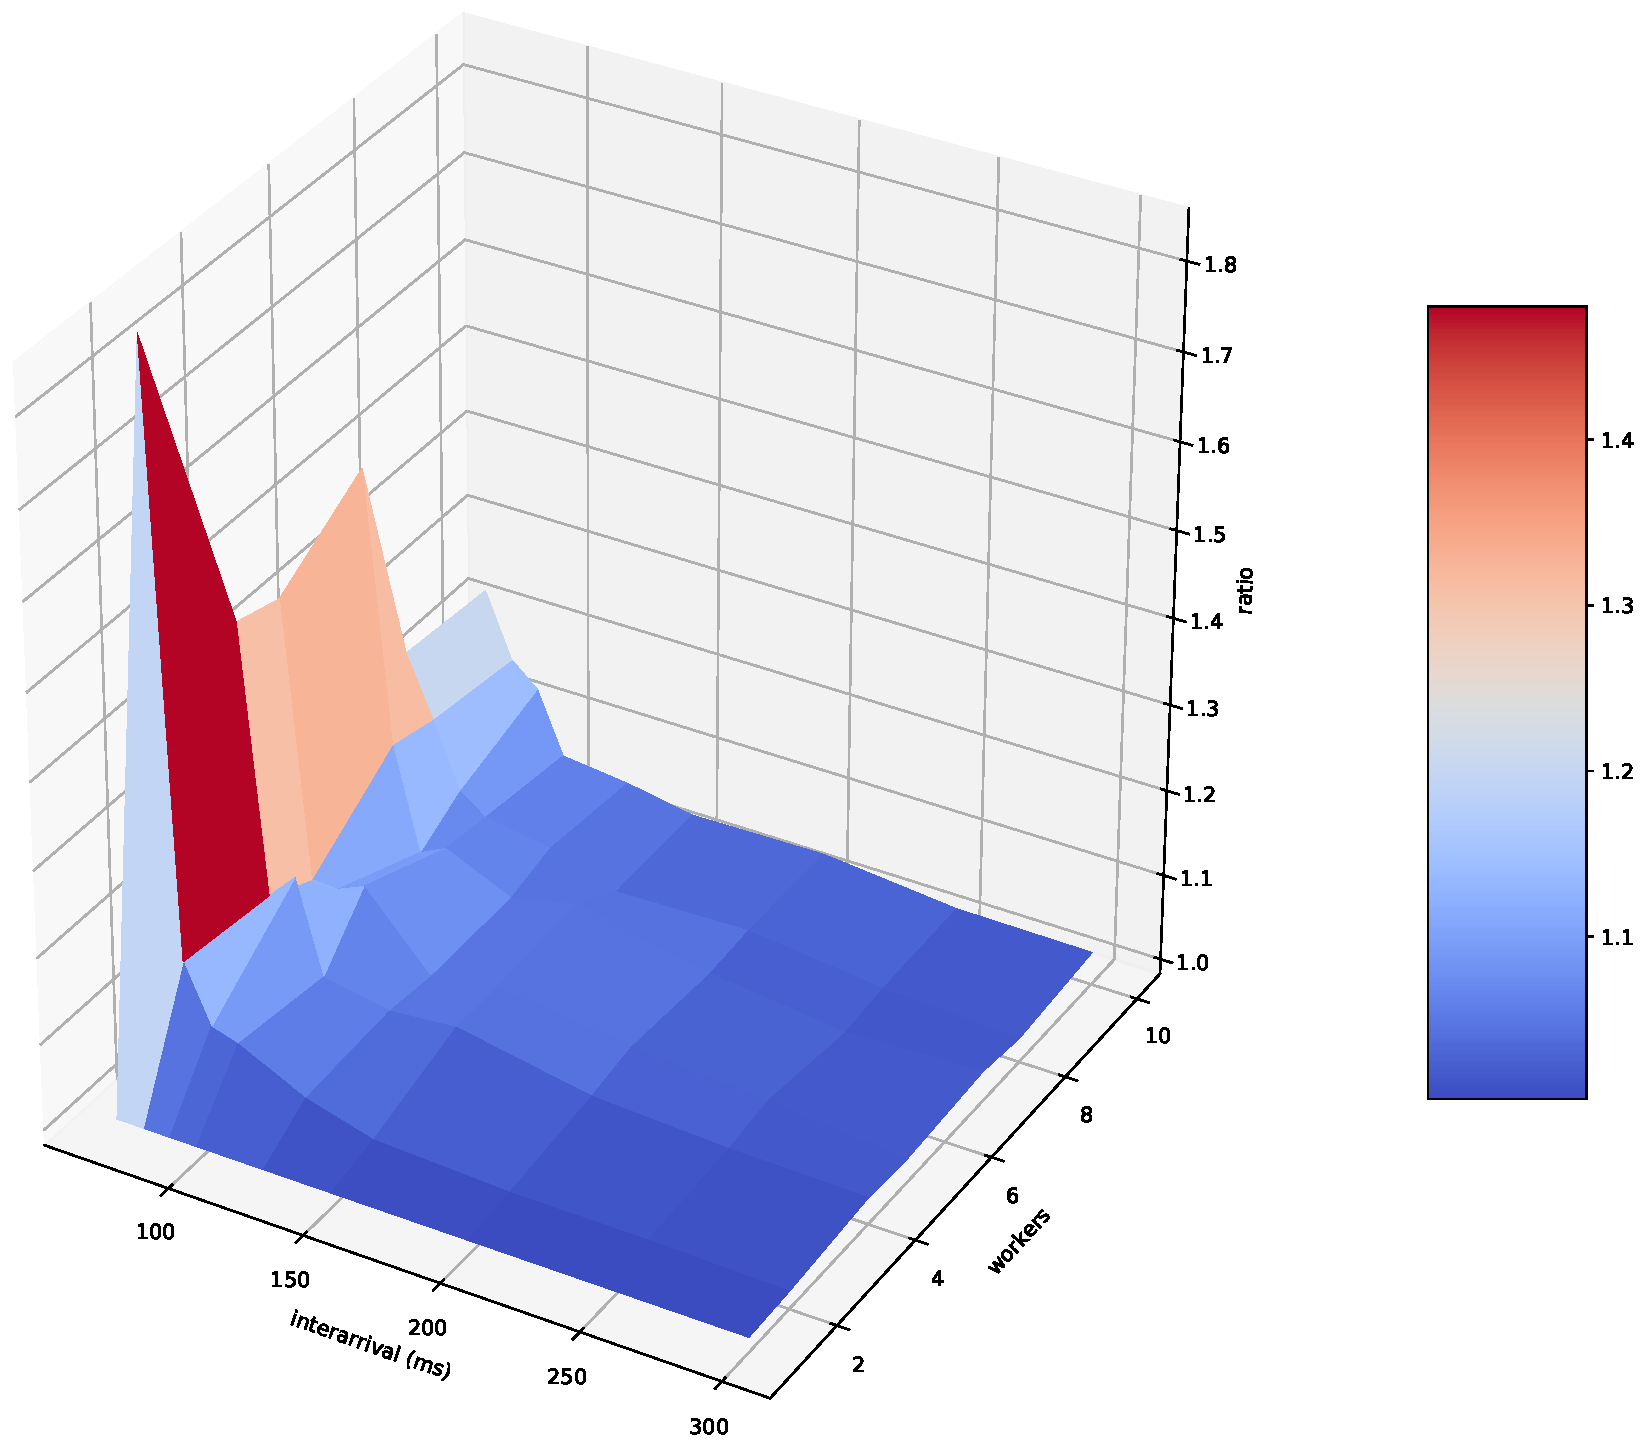
\includegraphics[width=0.48\textwidth]{pics/experiment}
  \caption{Experiment results}
  \label {experiment}
\end{figure}


\section{Related work}
%%% fs-seim-related - Related work

Seems to be related: \cite{4279071}, \cite{Wei:2009:SSO:1559845.1559973}, \cite{Mutschler:2014:ASP:2659232.2633686}.


\section{Conslusion}
%%% fs-seim-conclusion - Conclusion

\label {fs-conclusion}

In this paper we introduce an optimistic approach for handling out-of-order events. Our technique has the following key properties:

\begin{itemize}
    \item It does not require buffering before each order-sensitive operation
    \item The method handles properly any statful operation
    \item The overhead of the proposed approach is low and was under 10\% in most of our experiments
    \item The total overhead could be managed by optimization of the computational layout
\end{itemize}

The optimistic nature of this method is able to help to reduce the cost of waiting for punctuations or watermarks. It is implied by the fact, that at the moment when the watermark arrives all computations are already done. 

The experiments show that the number of the extra items does not increase with the growth of the number of the computational units. Therefore, this approach can potentially provide lower latency in stream processing systems.


\bibliographystyle{IEEEtran}
\bibliography{../../bibliography/flame-stream}

\end{document}

\endinput
